\documentclass{article}
\usepackage{graphicx}
\usepackage[letterpaper,textwidth=5in,right=2.5in,textheight=9in]{geometry}

\usepackage{amsmath,amssymb, changepage}
\usepackage{enumerate}
\usepackage{upgreek}
\pagestyle{empty}
\usepackage{listings}
\usepackage{tikz}
\begin{document}
\noindent
Joshua Kloepfer\\
9/30/2025\\
\textbf{Meshfields DOF Holder and Integration Point Ordering}\\\\
Linear Triangle:\\
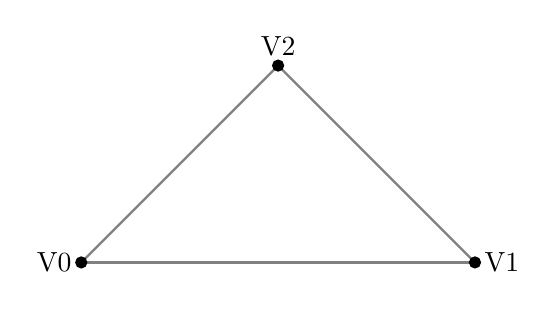
\begin{tikzpicture}
    \draw[gray, thick] (0, 0) -- (2.5, 2.5);
    \draw[gray, thick] (0, 0) -- (5, 0);
    \draw[gray, thick] (2.5, 2.5) -- (5, 0);
    \filldraw[black] (0, 0) circle (2pt) node[anchor=east]{V0};
    \filldraw[black] (5, 0) circle (2pt) node[anchor=west]{V1};
    \filldraw[black] (2.5, 2.5) circle (2pt) node[anchor=south]{V2};
\end{tikzpicture}
\\
Quadratic Triangle\\
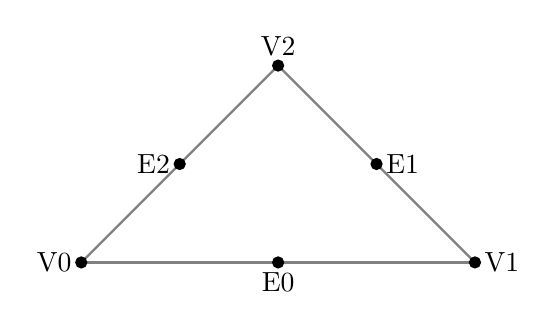
\begin{tikzpicture}
    \draw[gray, thick] (0, 0) -- (2.5, 2.5);
    \draw[gray, thick] (0, 0) -- (5, 0);
    \draw[gray, thick] (2.5, 2.5) -- (5, 0);
    \filldraw[black] (0, 0) circle (2pt) node[anchor=east]{V0};
    \filldraw[black] (5, 0) circle (2pt) node[anchor=west]{V1};
    \filldraw[black] (2.5, 2.5) circle (2pt) node[anchor=south]{V2};
    \filldraw[black] (2.5, 0) circle (2pt) node[anchor=north]{E0};
    \filldraw[black] (3.75, 1.25) circle (2pt) node[anchor=west]{E1};
    \filldraw[black] (1.25, 1.25) circle (2pt) node[anchor=east]{E2};
\end{tikzpicture}
\\
Linear Tetrahedron:\\
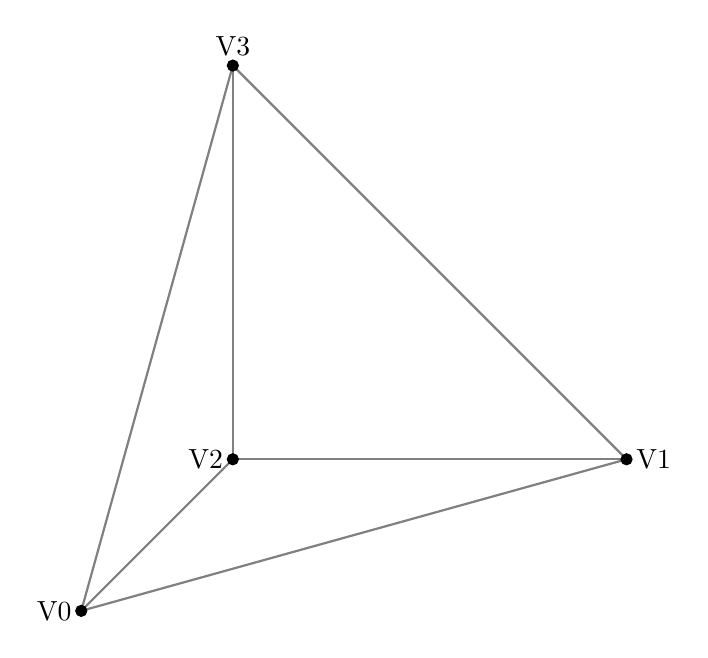
\begin{tikzpicture}
    \draw[gray, thick] (0, 0, 0) -- (5, 0, 0);
    \draw[gray, thick] (0, 0, 0) -- (0, 5, 0);
    \draw[gray, thick] (5, 0, 0) -- (0, 5, 0);
    \draw[gray, thick] (0, 0, 0) -- (0, 0, 5);
    \draw[gray, thick] (5, 0, 0) -- (0, 0, 5);
    \draw[gray, thick] (0, 5, 0) -- (0, 0, 5);
    \filldraw[black] (0, 0, 5) circle (2pt) node[anchor=east]{V0};
    \filldraw[black] (5, 0, 0) circle (2pt) node[anchor=west]{V1};
    \filldraw[black] (0, 0, 0) circle (2pt) node[anchor=east]{V2};
    \filldraw[black] (0, 5, 0) circle (2pt) node[anchor=south]{V3};
\end{tikzpicture}
\\
Vertex ordering must follow right hand rule.\\
Quadratic Tetrahedron:\\
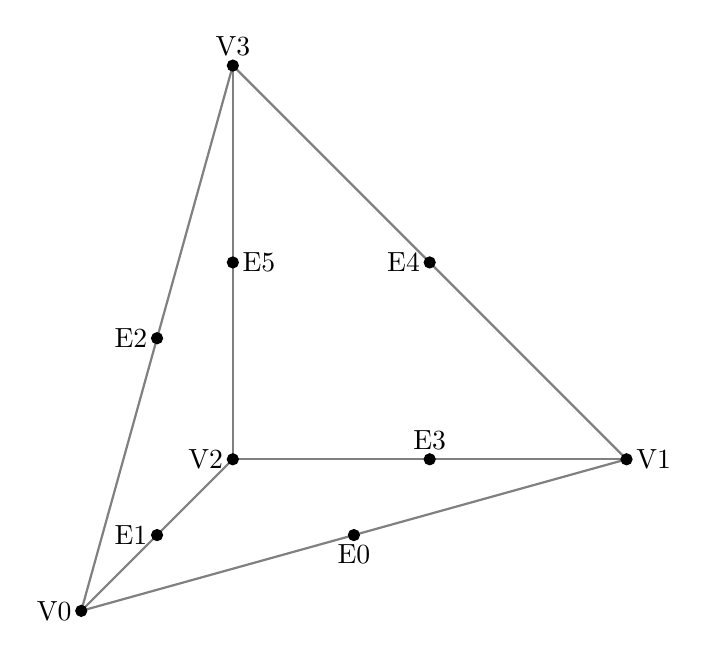
\begin{tikzpicture}
    \draw[gray, thick] (0, 0, 0) -- (5, 0, 0);
    \draw[gray, thick] (0, 0, 0) -- (0, 5, 0);
    \draw[gray, thick] (5, 0, 0) -- (0, 5, 0);
    \draw[gray, thick] (0, 0, 0) -- (0, 0, 5);
    \draw[gray, thick] (5, 0, 0) -- (0, 0, 5);
    \draw[gray, thick] (0, 5, 0) -- (0, 0, 5);
    \filldraw[black] (0, 0, 5) circle (2pt) node[anchor=east]{V0};
    \filldraw[black] (5, 0, 0) circle (2pt) node[anchor=west]{V1};
    \filldraw[black] (0, 0, 0) circle (2pt) node[anchor=east]{V2};
    \filldraw[black] (0, 5, 0) circle (2pt) node[anchor=south]{V3};
    
    \filldraw[black] (2.5, 0, 2.5) circle (2pt) node[anchor=north]{E0};
    \filldraw[black] (0, 0, 2.5) circle (2pt) node[anchor=east]{E1};
    \filldraw[black] (0, 2.5, 2.5) circle (2pt) node[anchor=east]{E2};
    \filldraw[black] (2.5, 0, 0) circle (2pt) node[anchor=south]{E3};
    \filldraw[black] (2.5, 2.5, 0) circle (2pt) node[anchor=east]{E4};
    \filldraw[black] (0, 2.5, 0) circle (2pt) node[anchor=west]{E5};
\end{tikzpicture}
\\
Vertex ordering must follow right hand rule and edge ordering must follow diagram.
\end{document}
